\subsection{Exact points: the observed reach in experiment E2}
Experiment E2 runs the same crop rotation and weather with one suction trigger at a time. Each dot is one run: its trigger and the irrigation it brought per year.
\begin{center}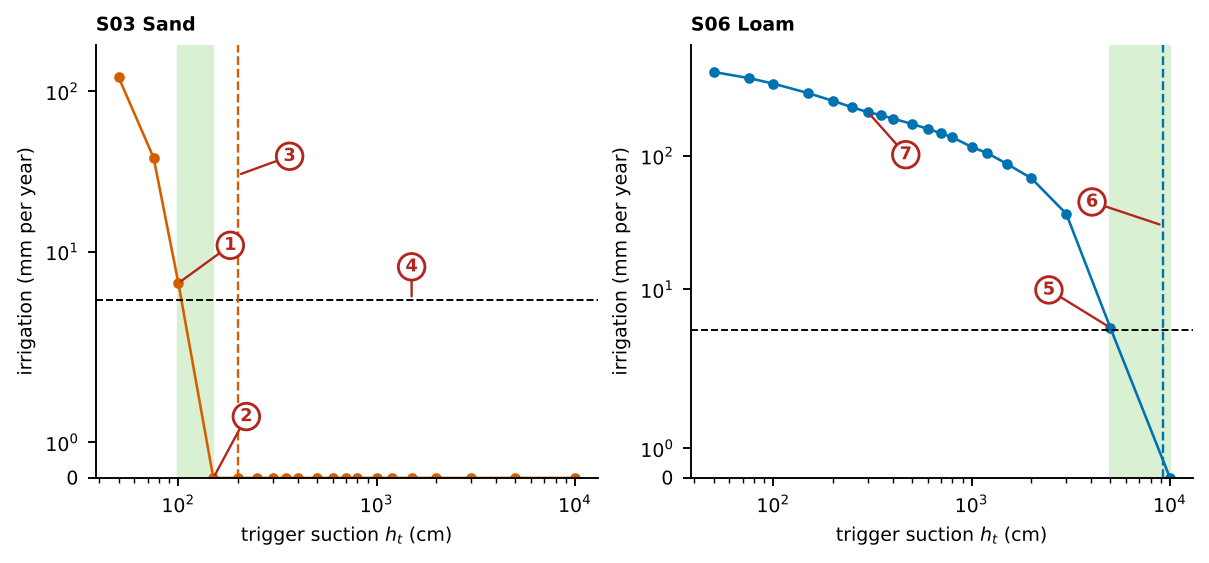
\includegraphics[width=0.92\textwidth]{../figures/paper4/ex_e2.png}\end{center}
\textbf{What the numbered labels point to, with the exact values.}
\begin{enumerate}[nosep,label=\protect\circled{\arabic*}]
\item Sand, the driest trigger that still fires: 100\,cm brings 6.36\,mm a year, above the 5\,mm line.
\item Sand, the next trigger, 150\,cm, brings 0.0\,mm: it never fires. The observed reach lies between the two (green band, 100--150\,cm).
\item The reach predicted by the closed form, 199\,cm (dashed): a third above the band, the largest miss among the soils with a finite interval.
\item The 5\,mm a year threshold that defines ``fires; with 1, 10, 20 or 40\,mm the fitted $\kappa$ becomes 2.7, 7.3, 13 or 25 $\times10^{-10}$.
\item Loam, the driest trigger that fires: 5000\,cm brings 5.16\,mm a year.
\item Predicted reach of loam, 9\,209\,cm: inside the observed band 5\,000--10\,000\,cm.
\item Loam at the usual 300\,cm trigger: 212\,mm a year of irrigation, the trigger works.
\end{enumerate}
\textbf{How the exact points are obtained from the data.} E2 is the experiment \texttt{E2\_TriggerPressure} of \nolinkurl{Data/Comprehensive_Summary/00_summary_all_simulations.csv.gz}: 10 soils $\times$ 20 triggers (20 to 10\,000\,cm), sensor at 20\,cm, dose 2.4\,mm, crop file \texttt{crops\_conv\_N100.dai}, weather Taastrup 1980--1999. For each soil the script \nolinkurl{p4_reach.py} takes the column \texttt{set\_trigger\_potential\_cm} (sign changed) and \texttt{irrigation\_mm}; the largest trigger with at least 5\,mm a year is the lower end of the interval, the next larger trigger the upper end. These points are in \nolinkurl{p4_fig3_trigger_runs.csv}.
